\documentclass[11pt]{article}

    \usepackage[breakable]{tcolorbox}
    \usepackage{parskip} % Stop auto-indenting (to mimic markdown behaviour)
    
    \usepackage{iftex}
    \ifPDFTeX
    	\usepackage[T1]{fontenc}
    	\usepackage{mathpazo}
    \else
    	\usepackage{fontspec}
    \fi

    % Basic figure setup, for now with no caption control since it's done
    % automatically by Pandoc (which extracts ![](path) syntax from Markdown).
    \usepackage{graphicx}
    % Maintain compatibility with old templates. Remove in nbconvert 6.0
    \let\Oldincludegraphics\includegraphics
    % Ensure that by default, figures have no caption (until we provide a
    % proper Figure object with a Caption API and a way to capture that
    % in the conversion process - todo).
    \usepackage{caption}
    \DeclareCaptionFormat{nocaption}{}
    \captionsetup{format=nocaption,aboveskip=0pt,belowskip=0pt}

    \usepackage[Export]{adjustbox} % Used to constrain images to a maximum size
    \adjustboxset{max size={0.9\linewidth}{0.9\paperheight}}
    \usepackage{float}
    \floatplacement{figure}{H} % forces figures to be placed at the correct location
    \usepackage{xcolor} % Allow colors to be defined
    \usepackage{enumerate} % Needed for markdown enumerations to work
    \usepackage{geometry} % Used to adjust the document margins
    \usepackage{amsmath} % Equations
    \usepackage{amssymb} % Equations
    \usepackage{textcomp} % defines textquotesingle
    % Hack from http://tex.stackexchange.com/a/47451/13684:
    \AtBeginDocument{%
        \def\PYZsq{\textquotesingle}% Upright quotes in Pygmentized code
    }
    \usepackage{upquote} % Upright quotes for verbatim code
    \usepackage{eurosym} % defines \euro
    \usepackage[mathletters]{ucs} % Extended unicode (utf-8) support
    \usepackage{fancyvrb} % verbatim replacement that allows latex
    \usepackage{grffile} % extends the file name processing of package graphics 
                         % to support a larger range
    \makeatletter % fix for grffile with XeLaTeX
    \def\Gread@@xetex#1{%
      \IfFileExists{"\Gin@base".bb}%
      {\Gread@eps{\Gin@base.bb}}%
      {\Gread@@xetex@aux#1}%
    }
    \makeatother

    % The hyperref package gives us a pdf with properly built
    % internal navigation ('pdf bookmarks' for the table of contents,
    % internal cross-reference links, web links for URLs, etc.)
    \usepackage{hyperref}
    % The default LaTeX title has an obnoxious amount of whitespace. By default,
    % titling removes some of it. It also provides customization options.
    \usepackage{titling}
    \usepackage{longtable} % longtable support required by pandoc >1.10
    \usepackage{booktabs}  % table support for pandoc > 1.12.2
    \usepackage[inline]{enumitem} % IRkernel/repr support (it uses the enumerate* environment)
    \usepackage[normalem]{ulem} % ulem is needed to support strikethroughs (\sout)
                                % normalem makes italics be italics, not underlines
    \usepackage{mathrsfs}
    

    
    % Colors for the hyperref package
    \definecolor{urlcolor}{rgb}{0,.145,.698}
    \definecolor{linkcolor}{rgb}{.71,0.21,0.01}
    \definecolor{citecolor}{rgb}{.12,.54,.11}

    % ANSI colors
    \definecolor{ansi-black}{HTML}{3E424D}
    \definecolor{ansi-black-intense}{HTML}{282C36}
    \definecolor{ansi-red}{HTML}{E75C58}
    \definecolor{ansi-red-intense}{HTML}{B22B31}
    \definecolor{ansi-green}{HTML}{00A250}
    \definecolor{ansi-green-intense}{HTML}{007427}
    \definecolor{ansi-yellow}{HTML}{DDB62B}
    \definecolor{ansi-yellow-intense}{HTML}{B27D12}
    \definecolor{ansi-blue}{HTML}{208FFB}
    \definecolor{ansi-blue-intense}{HTML}{0065CA}
    \definecolor{ansi-magenta}{HTML}{D160C4}
    \definecolor{ansi-magenta-intense}{HTML}{A03196}
    \definecolor{ansi-cyan}{HTML}{60C6C8}
    \definecolor{ansi-cyan-intense}{HTML}{258F8F}
    \definecolor{ansi-white}{HTML}{C5C1B4}
    \definecolor{ansi-white-intense}{HTML}{A1A6B2}
    \definecolor{ansi-default-inverse-fg}{HTML}{FFFFFF}
    \definecolor{ansi-default-inverse-bg}{HTML}{000000}

    % commands and environments needed by pandoc snippets
    % extracted from the output of `pandoc -s`
    \providecommand{\tightlist}{%
      \setlength{\itemsep}{0pt}\setlength{\parskip}{0pt}}
    \DefineVerbatimEnvironment{Highlighting}{Verbatim}{commandchars=\\\{\}}
    % Add ',fontsize=\small' for more characters per line
    \newenvironment{Shaded}{}{}
    \newcommand{\KeywordTok}[1]{\textcolor[rgb]{0.00,0.44,0.13}{\textbf{{#1}}}}
    \newcommand{\DataTypeTok}[1]{\textcolor[rgb]{0.56,0.13,0.00}{{#1}}}
    \newcommand{\DecValTok}[1]{\textcolor[rgb]{0.25,0.63,0.44}{{#1}}}
    \newcommand{\BaseNTok}[1]{\textcolor[rgb]{0.25,0.63,0.44}{{#1}}}
    \newcommand{\FloatTok}[1]{\textcolor[rgb]{0.25,0.63,0.44}{{#1}}}
    \newcommand{\CharTok}[1]{\textcolor[rgb]{0.25,0.44,0.63}{{#1}}}
    \newcommand{\StringTok}[1]{\textcolor[rgb]{0.25,0.44,0.63}{{#1}}}
    \newcommand{\CommentTok}[1]{\textcolor[rgb]{0.38,0.63,0.69}{\textit{{#1}}}}
    \newcommand{\OtherTok}[1]{\textcolor[rgb]{0.00,0.44,0.13}{{#1}}}
    \newcommand{\AlertTok}[1]{\textcolor[rgb]{1.00,0.00,0.00}{\textbf{{#1}}}}
    \newcommand{\FunctionTok}[1]{\textcolor[rgb]{0.02,0.16,0.49}{{#1}}}
    \newcommand{\RegionMarkerTok}[1]{{#1}}
    \newcommand{\ErrorTok}[1]{\textcolor[rgb]{1.00,0.00,0.00}{\textbf{{#1}}}}
    \newcommand{\NormalTok}[1]{{#1}}
    
    % Additional commands for more recent versions of Pandoc
    \newcommand{\ConstantTok}[1]{\textcolor[rgb]{0.53,0.00,0.00}{{#1}}}
    \newcommand{\SpecialCharTok}[1]{\textcolor[rgb]{0.25,0.44,0.63}{{#1}}}
    \newcommand{\VerbatimStringTok}[1]{\textcolor[rgb]{0.25,0.44,0.63}{{#1}}}
    \newcommand{\SpecialStringTok}[1]{\textcolor[rgb]{0.73,0.40,0.53}{{#1}}}
    \newcommand{\ImportTok}[1]{{#1}}
    \newcommand{\DocumentationTok}[1]{\textcolor[rgb]{0.73,0.13,0.13}{\textit{{#1}}}}
    \newcommand{\AnnotationTok}[1]{\textcolor[rgb]{0.38,0.63,0.69}{\textbf{\textit{{#1}}}}}
    \newcommand{\CommentVarTok}[1]{\textcolor[rgb]{0.38,0.63,0.69}{\textbf{\textit{{#1}}}}}
    \newcommand{\VariableTok}[1]{\textcolor[rgb]{0.10,0.09,0.49}{{#1}}}
    \newcommand{\ControlFlowTok}[1]{\textcolor[rgb]{0.00,0.44,0.13}{\textbf{{#1}}}}
    \newcommand{\OperatorTok}[1]{\textcolor[rgb]{0.40,0.40,0.40}{{#1}}}
    \newcommand{\BuiltInTok}[1]{{#1}}
    \newcommand{\ExtensionTok}[1]{{#1}}
    \newcommand{\PreprocessorTok}[1]{\textcolor[rgb]{0.74,0.48,0.00}{{#1}}}
    \newcommand{\AttributeTok}[1]{\textcolor[rgb]{0.49,0.56,0.16}{{#1}}}
    \newcommand{\InformationTok}[1]{\textcolor[rgb]{0.38,0.63,0.69}{\textbf{\textit{{#1}}}}}
    \newcommand{\WarningTok}[1]{\textcolor[rgb]{0.38,0.63,0.69}{\textbf{\textit{{#1}}}}}
    
    
    % Define a nice break command that doesn't care if a line doesn't already
    % exist.
    \def\br{\hspace*{\fill} \\* }
    % Math Jax compatibility definitions
    \def\gt{>}
    \def\lt{<}
    \let\Oldtex\TeX
    \let\Oldlatex\LaTeX
    \renewcommand{\TeX}{\textrm{\Oldtex}}
    \renewcommand{\LaTeX}{\textrm{\Oldlatex}}
    % Document parameters
    % Document title
	\title{Tarea 3\\M\'etodos Num\'ericos}
    \author{Benjamin Rivera}
    
    
    
    
    
% Pygments definitions
\makeatletter
\def\PY@reset{\let\PY@it=\relax \let\PY@bf=\relax%
    \let\PY@ul=\relax \let\PY@tc=\relax%
    \let\PY@bc=\relax \let\PY@ff=\relax}
\def\PY@tok#1{\csname PY@tok@#1\endcsname}
\def\PY@toks#1+{\ifx\relax#1\empty\else%
    \PY@tok{#1}\expandafter\PY@toks\fi}
\def\PY@do#1{\PY@bc{\PY@tc{\PY@ul{%
    \PY@it{\PY@bf{\PY@ff{#1}}}}}}}
\def\PY#1#2{\PY@reset\PY@toks#1+\relax+\PY@do{#2}}

\expandafter\def\csname PY@tok@w\endcsname{\def\PY@tc##1{\textcolor[rgb]{0.73,0.73,0.73}{##1}}}
\expandafter\def\csname PY@tok@c\endcsname{\let\PY@it=\textit\def\PY@tc##1{\textcolor[rgb]{0.25,0.50,0.50}{##1}}}
\expandafter\def\csname PY@tok@cp\endcsname{\def\PY@tc##1{\textcolor[rgb]{0.74,0.48,0.00}{##1}}}
\expandafter\def\csname PY@tok@k\endcsname{\let\PY@bf=\textbf\def\PY@tc##1{\textcolor[rgb]{0.00,0.50,0.00}{##1}}}
\expandafter\def\csname PY@tok@kp\endcsname{\def\PY@tc##1{\textcolor[rgb]{0.00,0.50,0.00}{##1}}}
\expandafter\def\csname PY@tok@kt\endcsname{\def\PY@tc##1{\textcolor[rgb]{0.69,0.00,0.25}{##1}}}
\expandafter\def\csname PY@tok@o\endcsname{\def\PY@tc##1{\textcolor[rgb]{0.40,0.40,0.40}{##1}}}
\expandafter\def\csname PY@tok@ow\endcsname{\let\PY@bf=\textbf\def\PY@tc##1{\textcolor[rgb]{0.67,0.13,1.00}{##1}}}
\expandafter\def\csname PY@tok@nb\endcsname{\def\PY@tc##1{\textcolor[rgb]{0.00,0.50,0.00}{##1}}}
\expandafter\def\csname PY@tok@nf\endcsname{\def\PY@tc##1{\textcolor[rgb]{0.00,0.00,1.00}{##1}}}
\expandafter\def\csname PY@tok@nc\endcsname{\let\PY@bf=\textbf\def\PY@tc##1{\textcolor[rgb]{0.00,0.00,1.00}{##1}}}
\expandafter\def\csname PY@tok@nn\endcsname{\let\PY@bf=\textbf\def\PY@tc##1{\textcolor[rgb]{0.00,0.00,1.00}{##1}}}
\expandafter\def\csname PY@tok@ne\endcsname{\let\PY@bf=\textbf\def\PY@tc##1{\textcolor[rgb]{0.82,0.25,0.23}{##1}}}
\expandafter\def\csname PY@tok@nv\endcsname{\def\PY@tc##1{\textcolor[rgb]{0.10,0.09,0.49}{##1}}}
\expandafter\def\csname PY@tok@no\endcsname{\def\PY@tc##1{\textcolor[rgb]{0.53,0.00,0.00}{##1}}}
\expandafter\def\csname PY@tok@nl\endcsname{\def\PY@tc##1{\textcolor[rgb]{0.63,0.63,0.00}{##1}}}
\expandafter\def\csname PY@tok@ni\endcsname{\let\PY@bf=\textbf\def\PY@tc##1{\textcolor[rgb]{0.60,0.60,0.60}{##1}}}
\expandafter\def\csname PY@tok@na\endcsname{\def\PY@tc##1{\textcolor[rgb]{0.49,0.56,0.16}{##1}}}
\expandafter\def\csname PY@tok@nt\endcsname{\let\PY@bf=\textbf\def\PY@tc##1{\textcolor[rgb]{0.00,0.50,0.00}{##1}}}
\expandafter\def\csname PY@tok@nd\endcsname{\def\PY@tc##1{\textcolor[rgb]{0.67,0.13,1.00}{##1}}}
\expandafter\def\csname PY@tok@s\endcsname{\def\PY@tc##1{\textcolor[rgb]{0.73,0.13,0.13}{##1}}}
\expandafter\def\csname PY@tok@sd\endcsname{\let\PY@it=\textit\def\PY@tc##1{\textcolor[rgb]{0.73,0.13,0.13}{##1}}}
\expandafter\def\csname PY@tok@si\endcsname{\let\PY@bf=\textbf\def\PY@tc##1{\textcolor[rgb]{0.73,0.40,0.53}{##1}}}
\expandafter\def\csname PY@tok@se\endcsname{\let\PY@bf=\textbf\def\PY@tc##1{\textcolor[rgb]{0.73,0.40,0.13}{##1}}}
\expandafter\def\csname PY@tok@sr\endcsname{\def\PY@tc##1{\textcolor[rgb]{0.73,0.40,0.53}{##1}}}
\expandafter\def\csname PY@tok@ss\endcsname{\def\PY@tc##1{\textcolor[rgb]{0.10,0.09,0.49}{##1}}}
\expandafter\def\csname PY@tok@sx\endcsname{\def\PY@tc##1{\textcolor[rgb]{0.00,0.50,0.00}{##1}}}
\expandafter\def\csname PY@tok@m\endcsname{\def\PY@tc##1{\textcolor[rgb]{0.40,0.40,0.40}{##1}}}
\expandafter\def\csname PY@tok@gh\endcsname{\let\PY@bf=\textbf\def\PY@tc##1{\textcolor[rgb]{0.00,0.00,0.50}{##1}}}
\expandafter\def\csname PY@tok@gu\endcsname{\let\PY@bf=\textbf\def\PY@tc##1{\textcolor[rgb]{0.50,0.00,0.50}{##1}}}
\expandafter\def\csname PY@tok@gd\endcsname{\def\PY@tc##1{\textcolor[rgb]{0.63,0.00,0.00}{##1}}}
\expandafter\def\csname PY@tok@gi\endcsname{\def\PY@tc##1{\textcolor[rgb]{0.00,0.63,0.00}{##1}}}
\expandafter\def\csname PY@tok@gr\endcsname{\def\PY@tc##1{\textcolor[rgb]{1.00,0.00,0.00}{##1}}}
\expandafter\def\csname PY@tok@ge\endcsname{\let\PY@it=\textit}
\expandafter\def\csname PY@tok@gs\endcsname{\let\PY@bf=\textbf}
\expandafter\def\csname PY@tok@gp\endcsname{\let\PY@bf=\textbf\def\PY@tc##1{\textcolor[rgb]{0.00,0.00,0.50}{##1}}}
\expandafter\def\csname PY@tok@go\endcsname{\def\PY@tc##1{\textcolor[rgb]{0.53,0.53,0.53}{##1}}}
\expandafter\def\csname PY@tok@gt\endcsname{\def\PY@tc##1{\textcolor[rgb]{0.00,0.27,0.87}{##1}}}
\expandafter\def\csname PY@tok@err\endcsname{\def\PY@bc##1{\setlength{\fboxsep}{0pt}\fcolorbox[rgb]{1.00,0.00,0.00}{1,1,1}{\strut ##1}}}
\expandafter\def\csname PY@tok@kc\endcsname{\let\PY@bf=\textbf\def\PY@tc##1{\textcolor[rgb]{0.00,0.50,0.00}{##1}}}
\expandafter\def\csname PY@tok@kd\endcsname{\let\PY@bf=\textbf\def\PY@tc##1{\textcolor[rgb]{0.00,0.50,0.00}{##1}}}
\expandafter\def\csname PY@tok@kn\endcsname{\let\PY@bf=\textbf\def\PY@tc##1{\textcolor[rgb]{0.00,0.50,0.00}{##1}}}
\expandafter\def\csname PY@tok@kr\endcsname{\let\PY@bf=\textbf\def\PY@tc##1{\textcolor[rgb]{0.00,0.50,0.00}{##1}}}
\expandafter\def\csname PY@tok@bp\endcsname{\def\PY@tc##1{\textcolor[rgb]{0.00,0.50,0.00}{##1}}}
\expandafter\def\csname PY@tok@fm\endcsname{\def\PY@tc##1{\textcolor[rgb]{0.00,0.00,1.00}{##1}}}
\expandafter\def\csname PY@tok@vc\endcsname{\def\PY@tc##1{\textcolor[rgb]{0.10,0.09,0.49}{##1}}}
\expandafter\def\csname PY@tok@vg\endcsname{\def\PY@tc##1{\textcolor[rgb]{0.10,0.09,0.49}{##1}}}
\expandafter\def\csname PY@tok@vi\endcsname{\def\PY@tc##1{\textcolor[rgb]{0.10,0.09,0.49}{##1}}}
\expandafter\def\csname PY@tok@vm\endcsname{\def\PY@tc##1{\textcolor[rgb]{0.10,0.09,0.49}{##1}}}
\expandafter\def\csname PY@tok@sa\endcsname{\def\PY@tc##1{\textcolor[rgb]{0.73,0.13,0.13}{##1}}}
\expandafter\def\csname PY@tok@sb\endcsname{\def\PY@tc##1{\textcolor[rgb]{0.73,0.13,0.13}{##1}}}
\expandafter\def\csname PY@tok@sc\endcsname{\def\PY@tc##1{\textcolor[rgb]{0.73,0.13,0.13}{##1}}}
\expandafter\def\csname PY@tok@dl\endcsname{\def\PY@tc##1{\textcolor[rgb]{0.73,0.13,0.13}{##1}}}
\expandafter\def\csname PY@tok@s2\endcsname{\def\PY@tc##1{\textcolor[rgb]{0.73,0.13,0.13}{##1}}}
\expandafter\def\csname PY@tok@sh\endcsname{\def\PY@tc##1{\textcolor[rgb]{0.73,0.13,0.13}{##1}}}
\expandafter\def\csname PY@tok@s1\endcsname{\def\PY@tc##1{\textcolor[rgb]{0.73,0.13,0.13}{##1}}}
\expandafter\def\csname PY@tok@mb\endcsname{\def\PY@tc##1{\textcolor[rgb]{0.40,0.40,0.40}{##1}}}
\expandafter\def\csname PY@tok@mf\endcsname{\def\PY@tc##1{\textcolor[rgb]{0.40,0.40,0.40}{##1}}}
\expandafter\def\csname PY@tok@mh\endcsname{\def\PY@tc##1{\textcolor[rgb]{0.40,0.40,0.40}{##1}}}
\expandafter\def\csname PY@tok@mi\endcsname{\def\PY@tc##1{\textcolor[rgb]{0.40,0.40,0.40}{##1}}}
\expandafter\def\csname PY@tok@il\endcsname{\def\PY@tc##1{\textcolor[rgb]{0.40,0.40,0.40}{##1}}}
\expandafter\def\csname PY@tok@mo\endcsname{\def\PY@tc##1{\textcolor[rgb]{0.40,0.40,0.40}{##1}}}
\expandafter\def\csname PY@tok@ch\endcsname{\let\PY@it=\textit\def\PY@tc##1{\textcolor[rgb]{0.25,0.50,0.50}{##1}}}
\expandafter\def\csname PY@tok@cm\endcsname{\let\PY@it=\textit\def\PY@tc##1{\textcolor[rgb]{0.25,0.50,0.50}{##1}}}
\expandafter\def\csname PY@tok@cpf\endcsname{\let\PY@it=\textit\def\PY@tc##1{\textcolor[rgb]{0.25,0.50,0.50}{##1}}}
\expandafter\def\csname PY@tok@c1\endcsname{\let\PY@it=\textit\def\PY@tc##1{\textcolor[rgb]{0.25,0.50,0.50}{##1}}}
\expandafter\def\csname PY@tok@cs\endcsname{\let\PY@it=\textit\def\PY@tc##1{\textcolor[rgb]{0.25,0.50,0.50}{##1}}}

\def\PYZbs{\char`\\}
\def\PYZus{\char`\_}
\def\PYZob{\char`\{}
\def\PYZcb{\char`\}}
\def\PYZca{\char`\^}
\def\PYZam{\char`\&}
\def\PYZlt{\char`\<}
\def\PYZgt{\char`\>}
\def\PYZsh{\char`\#}
\def\PYZpc{\char`\%}
\def\PYZdl{\char`\$}
\def\PYZhy{\char`\-}
\def\PYZsq{\char`\'}
\def\PYZdq{\char`\"}
\def\PYZti{\char`\~}
% for compatibility with earlier versions
\def\PYZat{@}
\def\PYZlb{[}
\def\PYZrb{]}
\makeatother


    % For linebreaks inside Verbatim environment from package fancyvrb. 
    \makeatletter
        \newbox\Wrappedcontinuationbox 
        \newbox\Wrappedvisiblespacebox 
        \newcommand*\Wrappedvisiblespace {\textcolor{red}{\textvisiblespace}} 
        \newcommand*\Wrappedcontinuationsymbol {\textcolor{red}{\llap{\tiny$\m@th\hookrightarrow$}}} 
        \newcommand*\Wrappedcontinuationindent {3ex } 
        \newcommand*\Wrappedafterbreak {\kern\Wrappedcontinuationindent\copy\Wrappedcontinuationbox} 
        % Take advantage of the already applied Pygments mark-up to insert 
        % potential linebreaks for TeX processing. 
        %        {, <, #, %, $, ' and ": go to next line. 
        %        _, }, ^, &, >, - and ~: stay at end of broken line. 
        % Use of \textquotesingle for straight quote. 
        \newcommand*\Wrappedbreaksatspecials {% 
            \def\PYGZus{\discretionary{\char`\_}{\Wrappedafterbreak}{\char`\_}}% 
            \def\PYGZob{\discretionary{}{\Wrappedafterbreak\char`\{}{\char`\{}}% 
            \def\PYGZcb{\discretionary{\char`\}}{\Wrappedafterbreak}{\char`\}}}% 
            \def\PYGZca{\discretionary{\char`\^}{\Wrappedafterbreak}{\char`\^}}% 
            \def\PYGZam{\discretionary{\char`\&}{\Wrappedafterbreak}{\char`\&}}% 
            \def\PYGZlt{\discretionary{}{\Wrappedafterbreak\char`\<}{\char`\<}}% 
            \def\PYGZgt{\discretionary{\char`\>}{\Wrappedafterbreak}{\char`\>}}% 
            \def\PYGZsh{\discretionary{}{\Wrappedafterbreak\char`\#}{\char`\#}}% 
            \def\PYGZpc{\discretionary{}{\Wrappedafterbreak\char`\%}{\char`\%}}% 
            \def\PYGZdl{\discretionary{}{\Wrappedafterbreak\char`\$}{\char`\$}}% 
            \def\PYGZhy{\discretionary{\char`\-}{\Wrappedafterbreak}{\char`\-}}% 
            \def\PYGZsq{\discretionary{}{\Wrappedafterbreak\textquotesingle}{\textquotesingle}}% 
            \def\PYGZdq{\discretionary{}{\Wrappedafterbreak\char`\"}{\char`\"}}% 
            \def\PYGZti{\discretionary{\char`\~}{\Wrappedafterbreak}{\char`\~}}% 
        } 
        % Some characters . , ; ? ! / are not pygmentized. 
        % This macro makes them "active" and they will insert potential linebreaks 
        \newcommand*\Wrappedbreaksatpunct {% 
            \lccode`\~`\.\lowercase{\def~}{\discretionary{\hbox{\char`\.}}{\Wrappedafterbreak}{\hbox{\char`\.}}}% 
            \lccode`\~`\,\lowercase{\def~}{\discretionary{\hbox{\char`\,}}{\Wrappedafterbreak}{\hbox{\char`\,}}}% 
            \lccode`\~`\;\lowercase{\def~}{\discretionary{\hbox{\char`\;}}{\Wrappedafterbreak}{\hbox{\char`\;}}}% 
            \lccode`\~`\:\lowercase{\def~}{\discretionary{\hbox{\char`\:}}{\Wrappedafterbreak}{\hbox{\char`\:}}}% 
            \lccode`\~`\?\lowercase{\def~}{\discretionary{\hbox{\char`\?}}{\Wrappedafterbreak}{\hbox{\char`\?}}}% 
            \lccode`\~`\!\lowercase{\def~}{\discretionary{\hbox{\char`\!}}{\Wrappedafterbreak}{\hbox{\char`\!}}}% 
            \lccode`\~`\/\lowercase{\def~}{\discretionary{\hbox{\char`\/}}{\Wrappedafterbreak}{\hbox{\char`\/}}}% 
            \catcode`\.\active
            \catcode`\,\active 
            \catcode`\;\active
            \catcode`\:\active
            \catcode`\?\active
            \catcode`\!\active
            \catcode`\/\active 
            \lccode`\~`\~ 	
        }
    \makeatother

    \let\OriginalVerbatim=\Verbatim
    \makeatletter
    \renewcommand{\Verbatim}[1][1]{%
        %\parskip\z@skip
        \sbox\Wrappedcontinuationbox {\Wrappedcontinuationsymbol}%
        \sbox\Wrappedvisiblespacebox {\FV@SetupFont\Wrappedvisiblespace}%
        \def\FancyVerbFormatLine ##1{\hsize\linewidth
            \vtop{\raggedright\hyphenpenalty\z@\exhyphenpenalty\z@
                \doublehyphendemerits\z@\finalhyphendemerits\z@
                \strut ##1\strut}%
        }%
        % If the linebreak is at a space, the latter will be displayed as visible
        % space at end of first line, and a continuation symbol starts next line.
        % Stretch/shrink are however usually zero for typewriter font.
        \def\FV@Space {%
            \nobreak\hskip\z@ plus\fontdimen3\font minus\fontdimen4\font
            \discretionary{\copy\Wrappedvisiblespacebox}{\Wrappedafterbreak}
            {\kern\fontdimen2\font}%
        }%
        
        % Allow breaks at special characters using \PYG... macros.
        \Wrappedbreaksatspecials
        % Breaks at punctuation characters . , ; ? ! and / need catcode=\active 	
        \OriginalVerbatim[#1,codes*=\Wrappedbreaksatpunct]%
    }
    \makeatother

    % Exact colors from NB
    \definecolor{incolor}{HTML}{303F9F}
    \definecolor{outcolor}{HTML}{D84315}
    \definecolor{cellborder}{HTML}{CFCFCF}
    \definecolor{cellbackground}{HTML}{F7F7F7}
    
    % prompt
    \makeatletter
    \newcommand{\boxspacing}{\kern\kvtcb@left@rule\kern\kvtcb@boxsep}
    \makeatother
    \newcommand{\prompt}[4]{
        \ttfamily\llap{{\color{#2}[#3]:\hspace{3pt}#4}}\vspace{-\baselineskip}
    }
    

    
    % Prevent overflowing lines due to hard-to-break entities
    \sloppy 
    % Setup hyperref package
    \hypersetup{
      breaklinks=true,  % so long urls are correctly broken across lines
      colorlinks=true,
      urlcolor=urlcolor,
      linkcolor=linkcolor,
      citecolor=citecolor,
      }
    % Slightly bigger margins than the latex defaults
    
    \usepackage[spanish]{babel}
    \usepackage{multicol}
    
    
    \geometry{tmargin=0.5in, bmargin=0.7in, lmargin=0.45in, rmargin=2.5in}
    
    
\begin{document}
    
    \maketitle
    \tableofcontents

 
    

    \newpage
    \hypertarget{tarea-3}{%
\section{Tarea 3}\label{tarea-3}}

\emph{Tarea 3} de \emph{Benjamín Rivera} para el curso de
\textbf{Métodos Numéricos} impartido por \emph{Joaquín Peña Acevedo}.
Fecha limite de entrega \textbf{20 de Septiembre de 2020}.

    \hypertarget{como-ejecutar}{%
\subsubsection{Como ejecutar}\label{como-ejecutar}}

    \hypertarget{requerimientos}{%
\subparagraph{Requerimientos}\label{requerimientos}}

Este programa se ejecuto en mi computadora con la version de
\textbf{Python 3.8.2} y con estos
\href{https://github.com/BenchHPZ/UG-Compu/blob/master/MN/requerimientos.txt}{requerimientos}

\hypertarget{jupyter}{%
\paragraph{Jupyter}\label{jupyter}}

En caso de tener acceso a un \emph{servidor jupyter} ,con los
requerimientos antes mencionados, unicamente basta con ejecutar todas
las celdas de este \emph{notebook}. Probablemente no todas las celdas de
\emph{markdown} produzcan el mismo resultado por las
\href{jupyter-contrib-nbextensions.readthedocs.io}{\emph{Nbextensions}}.

\hypertarget{consola}{%
\paragraph{Consola}\label{consola}}

Habrá archivos e instrucciones para poder ejecutar cada uno de los
ejercicios desde la consola.

\hypertarget{si-todo-sale-mal}{%
\paragraph{Si todo sale mal}\label{si-todo-sale-mal}}

En caso de que todo salga mal, tratare de dejar una copia disponible en
\href{https://colab.research.google.com/gist/BenchHPZ/813abd96c1dac91b038905ac85cc425c/tarea3.ipynb}{\bf GoogleColab} que se pueda ejecutar con su versión de
\textbf{Python}. Es imporante primero subir los archivos a la instancia local para que los pueda usar el programa.













\newpage
    \hypertarget{ejercicio-1}{%
\subsection{Ejercicio 1}\label{ejercicio-1}}

    \hypertarget{section}{%
\subsubsection{.}\label{section}}

Muestre que la inversa de \(L_k\) es \(L^{-1}_k = I + l_ke_k^T\). Asi,
la inversa de una matriz triangular inferior elemental es otra matriz
triangular inferior elemental.

    Sabemos que, si la matriz es invertible, entonces \(L_kL_k^{-1} = I\).

Procedemos por contradiccion. Supongamos que
\(L^{-1}_k \neq I + l_ke_k^T\), de manera que
\(L_k(I + l_ke_k^T) \neq I\); si desarrolamos lo anterior resulta que

\begin{eqnarray*}
    L_k(I + l_ke_k^T) &\neq& I \\
    (I - l_ke_k^T)(I + l_ke_k^T) &\neq& I \\
    I^2 - (l_ke_k^T)^2 &\neq& I \\
    I - (l_ke_k^T)^2 &\neq& I \\ 
\end{eqnarray*}

lo cual es cierto siempre que \((l_ke_k^T)^2 \neq \bar{0}\). Sin
embargo, por la manera en que estan definidas \(l_ke_k^T\),
\((l_ke_k^T)^2 = 0\). Por lo que llegamos auna contradicion y
\(L^{-1}_k = I + l_ke_k^T\).

    \hypertarget{section}{%
\subsubsection{.}\label{section}}

Muestre que \(L^{-1}_{k-1}L^{-1}_k = I + l_{k-1}e^T_k + l_ke^t_k\) y con
esto demostrar que

\begin{equation*} L = L^{-1}_1 L^{-1}_2 \dots L^{-1}_{n-1} = I + \sum_{k=1}^{n-1}l_ke_k^T
\end{equation*}

por lo que \(L\) es una matriz triangular inferior con 1's en la
diagonal

    \textbf{Parte 1} Por definicion y el punto anterior

\begin{eqnarray*}
    L_{k-1}^{-1}L_{k}^{-1} &=& (I + l_{k-1}e_{k-1}^T)(I + l_ke_k^T) \\
        &=& I^2 + l_{k-1}e_{k-1}^T(l_ke_k^T) + l_{k-1}e_{k-1}^T + l_ke_k^T \\
        &&\text{y como sabemos que la multiplicacion de las submatrices $l,e$ es 0} \\
        &=& I + \bar{0} + l_{k-1}e_{k-1}^T + l_ke_k^T \\
        &=& I + l_{k-1}e_{k-1}^T + l_ke_k^T 
\end{eqnarray*}

\textbf{Parte 2} \ldots{}















\newpage
    \hypertarget{ejercicio-2}{%
\subsection{Ejercicio 2}\label{ejercicio-2}}

    \begin{tcolorbox}[breakable, size=fbox, boxrule=1pt, pad at break*=1mm,colback=cellbackground, colframe=cellborder]
\prompt{In}{incolor}{2}{\boxspacing}
\begin{Verbatim}[commandchars=\\\{\}]
\PY{k}{def} \PY{n+nf}{show1D}\PY{p}{(} \PY{n}{x}\PY{p}{,}\PY{n}{sz}\PY{p}{,}\PY{o}{/}\PY{p}{,} \PY{n}{max\PYZus{}sz}\PY{o}{=}\PY{l+m+mi}{8}\PY{p}{,} \PY{n}{prnt}\PY{o}{=}\PY{k+kc}{True}\PY{p}{)}\PY{p}{:}
    \PY{l+s+sd}{\PYZdq{}\PYZdq{}\PYZdq{} Funcion que recibe un arreglo 1D y, en caso de}
\PY{l+s+sd}{    que no sea muy grande, lo imprime en pantalla. En}
\PY{l+s+sd}{    caso de que lo sea, imprime datos representativos.}
\PY{l+s+sd}{        Input:}
\PY{l+s+sd}{            x := Apuntador al arreglo 1D para imprimir}
\PY{l+s+sd}{            sz := Tamanio del arreglo. (para la imple\PYZus{}}
\PY{l+s+sd}{                mentacion en python es inecesario, pe\PYZus{}}
\PY{l+s+sd}{                ro lo solicita el ejercicio)}
\PY{l+s+sd}{            max\PYZus{}sz := Maximo de elementos a imprimir}
\PY{l+s+sd}{            prnt := Indica si el string obtenido se }
\PY{l+s+sd}{                debe imprimir en pantalla}
\PY{l+s+sd}{        Output:}
\PY{l+s+sd}{            Esta funcion regresa}
\PY{l+s+sd}{            }
\PY{l+s+sd}{        \PYZus{}Doctest:}
\PY{l+s+sd}{            \PYZgt{}\PYZgt{}\PYZgt{} show1D([1,2,3,8,5,6,7,8,9,0], 10, prnt=False)}
\PY{l+s+sd}{            \PYZsq{}1, 2, 3, 8, ... , 7, 8, 9, 0\PYZsq{}}
\PY{l+s+sd}{            }
\PY{l+s+sd}{            \PYZgt{}\PYZgt{}\PYZgt{} show1D([1,2,3,8], 4, prnt=False)}
\PY{l+s+sd}{            \PYZsq{}1, 2, 3, 8\PYZsq{}}
\PY{l+s+sd}{    \PYZdq{}\PYZdq{}\PYZdq{}}
    \PY{k}{return} \PY{n}{ret}       
\end{Verbatim}
\end{tcolorbox}

    \begin{tcolorbox}[breakable, size=fbox, boxrule=1pt, pad at break*=1mm,colback=cellbackground, colframe=cellborder]
\prompt{In}{incolor}{3}{\boxspacing}
\begin{Verbatim}[commandchars=\\\{\}]
\PY{k}{def} \PY{n+nf}{forwardSubstitution}\PY{p}{(} \PY{n}{L}\PY{p}{,} \PY{n}{n}\PY{p}{,} \PY{n}{b}\PY{p}{,} \PY{n}{t}\PY{p}{,}\PY{o}{/}\PY{p}{,}\PY{n}{dtype}\PY{o}{=}\PY{n}{np}\PY{o}{.}\PY{n}{float64}\PY{p}{)}\PY{p}{:}
    \PY{l+s+sd}{\PYZdq{}\PYZdq{}\PYZdq{} Funcion que implementa el metodo desustitucion pa\PYZus{}}
\PY{l+s+sd}{    ra adelante dada una matriz triangular inferior.}
\PY{l+s+sd}{        Input:}
\PY{l+s+sd}{            L := apuntador a la matriz L}
\PY{l+s+sd}{            n := tamanio de la matriz L}
\PY{l+s+sd}{            b := apuntador al vector b}
\PY{l+s+sd}{            t := tolerancia de 0\PYZsq{}s}
\PY{l+s+sd}{        Otput:}
\PY{l+s+sd}{            ret := vector x de respuestas si se encontro, o}
\PY{l+s+sd}{                None en caso de que hay habido algun error}
\PY{l+s+sd}{                }
\PY{l+s+sd}{        \PYZus{}Doctest:}
\PY{l+s+sd}{            \PYZgt{}\PYZgt{}\PYZgt{} forwardSubstitution(np.matrix([[1,0],[0,1]]), 1, np.matrix([[3,4]]), 0.1)}
\PY{l+s+sd}{            matrix([[3.],}
\PY{l+s+sd}{                    [4.]])}
\PY{l+s+sd}{    \PYZdq{}\PYZdq{}\PYZdq{}}

    \PY{k}{if} \PY{n+nb}{len}\PY{p}{(}\PY{n}{L}\PY{p}{)} \PY{o}{==} \PY{n}{b}\PY{o}{.}\PY{n}{size}\PY{p}{:}
        \PY{k}{return} \PY{n}{np}\PY{o}{.}\PY{n}{asmatrix}\PY{p}{(}\PY{n}{x}\PY{p}{,} \PY{n}{dtype}\PY{o}{=}\PY{n}{dtype}\PY{p}{)}\PY{o}{.}\PY{n}{transpose}\PY{p}{(}\PY{p}{)}
    \PY{k}{else}\PY{p}{:}
        \PY{k}{return} \PY{k+kc}{None}
\end{Verbatim}
\end{tcolorbox}

    \begin{tcolorbox}[breakable, size=fbox, boxrule=1pt, pad at break*=1mm,colback=cellbackground, colframe=cellborder]
\prompt{In}{incolor}{4}{\boxspacing}
\begin{Verbatim}[commandchars=\\\{\}]
\PY{k}{def} \PY{n+nf}{readFile}\PY{p}{(}\PY{n}{file}\PY{p}{,}\PY{o}{/}\PY{p}{,} \PY{n}{path}\PY{o}{=}\PY{l+s+s1}{\PYZsq{}}\PY{l+s+s1}{datos/npy/}\PY{l+s+s1}{\PYZsq{}}\PY{p}{,} \PY{n}{ext}\PY{o}{=}\PY{l+s+s1}{\PYZsq{}}\PY{l+s+s1}{.npy}\PY{l+s+s1}{\PYZsq{}}\PY{p}{,} \PY{n}{dtype}\PY{o}{=}\PY{n}{np}\PY{o}{.}\PY{n}{float64}\PY{p}{)}\PY{p}{:}
    \PY{k}{return} \PY{n}{np}\PY{o}{.}\PY{n}{asmatrix}\PY{p}{(}\PY{n}{np}\PY{o}{.}\PY{n}{load}\PY{p}{(}\PY{n}{file}\PY{o}{=} \PY{n+nb}{str}\PY{p}{(}\PY{n}{path}\PY{o}{+}\PY{n}{file}\PY{o}{+}\PY{n}{ext}\PY{p}{)}\PY{p}{,} 
  
  
\PY{k}{def} \PY{n+nf}{Ejercicio2}\PY{p}{(}\PY{n}{f\PYZus{}L}\PY{p}{,} \PY{n}{f\PYZus{}b}\PY{p}{)}\PY{p}{:}
    \PY{l+s+sd}{\PYZdq{}\PYZdq{}\PYZdq{} Programa para ejecutar el ejercicio 2. espera el nombre}
\PY{l+s+sd}{    de los archivos de la matriz y el vector soluciones para }
\PY{l+s+sd}{    funcionar.}
\PY{l+s+sd}{    \PYZdq{}\PYZdq{}\PYZdq{}}
    \PY{n}{L} \PY{o}{=} \PY{n}{readFile}\PY{p}{(}\PY{n}{f\PYZus{}L}\PY{p}{)}
    \PY{n}{b} \PY{o}{=} \PY{n}{readFile}\PY{p}{(}\PY{n}{f\PYZus{}b}\PY{p}{)}
    \PY{n}{dtype} \PY{o}{=} \PY{n}{np}\PY{o}{.}\PY{n}{float64}
    \PY{n}{t} \PY{o}{=} \PY{p}{(}\PY{l+m+mf}{2.2e\PYZhy{}16}\PY{p}{)}\PY{o}{*}\PY{o}{*}\PY{p}{(}\PY{l+m+mi}{2}\PY{o}{/}\PY{l+m+mi}{3}\PY{p}{)} \PY{c+c1}{\PYZsh{} De la tarea 1 y como estamos usando flaot64}

\PY{k}{if} \PY{n}{True}\PY{p}{:}    
    \PY{k}{for} \PY{n}{sz} \PY{o+ow}{in} \PY{p}{[}\PY{l+m+mi}{5}\PY{p}{,} \PY{l+m+mi}{50}\PY{p}{,} \PY{l+m+mi}{500}\PY{p}{]}\PY{p}{:}
        \PY{n}{Ejercicio2}\PY{p}{(}\PY{l+s+s1}{\PYZsq{}}\PY{l+s+s1}{matL}\PY{l+s+s1}{\PYZsq{}}\PY{o}{+}\PY{n+nb}{str}\PY{p}{(}\PY{n}{sz}\PY{p}{)}\PY{p}{,} \PY{l+s+s1}{\PYZsq{}}\PY{l+s+s1}{vecb}\PY{l+s+s1}{\PYZsq{}}\PY{o}{+}\PY{n+nb}{str}\PY{p}{(}\PY{n}{sz}\PY{p}{)}\PY{p}{)}
        \PY{n+nb}{print}\PY{p}{(}\PY{l+s+s1}{\PYZsq{}}\PY{l+s+se}{\PYZbs{}n}\PY{l+s+s1}{\PYZsq{}}\PY{p}{)}
\end{Verbatim}
\end{tcolorbox}

    \begin{Verbatim}[commandchars=\\\{\}]
5 5
[ 0.33006882]
 [-0.78428134]
 [ 0.70227498]
 [ 0.48272233]
 [-0.61319569]
Error =
 12.755173555608748


50 50
Err: 0 o casi cero en diagonal
El sistema no tiene solucion.
Y es singular.


500 500
[ 1.27622082]
 [ 1.39905809]
 [-3.80410368]
 [ 2.83344826], {\ldots} , [ 4.01907914e+110]
 [ 8.50132313e+110]
 [-6.48257593e+110]
 [ 1.66110939e+111]
Error =
 8.245074985591727e+111


    \end{Verbatim}

    \hypertarget{como-ejecutar}{%
\paragraph{Como ejecutar}\label{como-ejecutar}}

Para ejecutar en consola se necesita estar en el mismo directorio que la
carpeta de la tarea \texttt{datos}. Como nombre de los archivos no se
espera la direccion completa ni la extension del archivo. Se infiere
automatincamente que los datos sera obtenidos del subdirectorio
\texttt{datos/npy} y con la extension \texttt{.npy}. De manera qu la
ejecucion debe parecerse a lo siguiente

\begin{verbatim}
python3 Tarea3.py Ejercicio2 matL5 vecb5
\end{verbatim}

lo que debe producir la salida

\begin{figure}
\centering
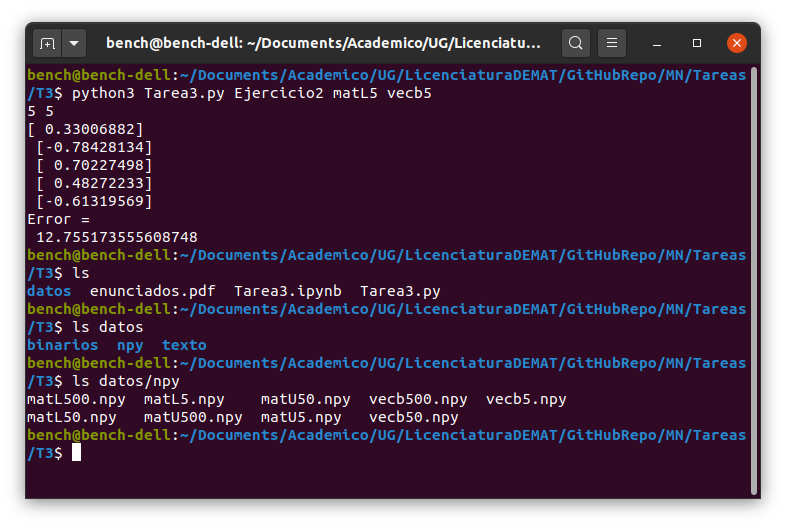
\includegraphics{assets/T3-E2.png}
\caption{Ejemplo ejecucion consola}
\end{figure}

\hypertarget{otros}{%
\paragraph{Otros}\label{otros}}

\href{https://numpy.org/doc/stable/reference/generated/numpy.linalg.norm.html}{Norma
de Numpy}















\newpage
    \hypertarget{ejercicio-3}{%
\subsection{Ejercicio 3}\label{ejercicio-3}}

    \begin{tcolorbox}[breakable, size=fbox, boxrule=1pt, pad at break*=1mm,colback=cellbackground, colframe=cellborder]
\prompt{In}{incolor}{5}{\boxspacing}
\begin{Verbatim}[commandchars=\\\{\}]
\PY{k}{def} \PY{n+nf}{backwardSubstitution}\PY{p}{(} \PY{n}{U}\PY{p}{,} \PY{n}{n}\PY{p}{,} \PY{n}{b}\PY{p}{,} \PY{n}{t}\PY{p}{,}\PY{o}{/}\PY{p}{,}\PY{n}{dtype}\PY{o}{=}\PY{n}{np}\PY{o}{.}\PY{n}{float64}\PY{p}{)}\PY{p}{:}
    \PY{l+s+sd}{\PYZdq{}\PYZdq{}\PYZdq{} Funcion que implementa el metodo desustitucion pa\PYZus{}}
\PY{l+s+sd}{    ra atras dada una matriz triangular inferior.}
\PY{l+s+sd}{        Input:}
\PY{l+s+sd}{            U := apuntador a la matriz U}
\PY{l+s+sd}{            n := tamanio de la matriz U}
\PY{l+s+sd}{            b := apuntador al vector b}
\PY{l+s+sd}{            t := tolerancia de 0\PYZsq{}s}
\PY{l+s+sd}{        Otput:}
\PY{l+s+sd}{            ret := vector x de respuestas si se encontro, o}
\PY{l+s+sd}{                None en caso de que hay habido algun error}
\PY{l+s+sd}{    \PYZdq{}\PYZdq{}\PYZdq{}}
        \PY{k}{return} \PY{k+kc}{None}
\end{Verbatim}
\end{tcolorbox}

    \begin{tcolorbox}[breakable, size=fbox, boxrule=1pt, pad at break*=1mm,colback=cellbackground, colframe=cellborder]
\prompt{In}{incolor}{8}{\boxspacing}
\begin{Verbatim}[commandchars=\\\{\}]
\PY{k}{def} \PY{n+nf}{Ejercicio3}\PY{p}{(}\PY{n}{f\PYZus{}U}\PY{p}{,} \PY{n}{f\PYZus{}b}\PY{p}{)}\PY{p}{:}
    \PY{l+s+sd}{\PYZdq{}\PYZdq{}\PYZdq{} Programa para ejecutar el ejercicio 3. espera el nombre}
\PY{l+s+sd}{    de los archivos de la matriz y el vector soluciones para }
\PY{l+s+sd}{    funcionar.}
\PY{l+s+sd}{    \PYZdq{}\PYZdq{}\PYZdq{}}

\PY{k}{if} \PY{n}{True}\PY{p}{:}    
    \PY{k}{for} \PY{n}{sz} \PY{o+ow}{in} \PY{p}{[}\PY{l+m+mi}{5}\PY{p}{,} \PY{l+m+mi}{50}\PY{p}{,} \PY{l+m+mi}{500}\PY{p}{]}\PY{p}{:}
        \PY{n}{Ejercicio3}\PY{p}{(}\PY{l+s+s1}{\PYZsq{}}\PY{l+s+s1}{matU}\PY{l+s+s1}{\PYZsq{}}\PY{o}{+}\PY{n+nb}{str}\PY{p}{(}\PY{n}{sz}\PY{p}{)}\PY{p}{,} \PY{l+s+s1}{\PYZsq{}}\PY{l+s+s1}{vecb}\PY{l+s+s1}{\PYZsq{}}\PY{o}{+}\PY{n+nb}{str}\PY{p}{(}\PY{n}{sz}\PY{p}{)}\PY{p}{)}
        \PY{n+nb}{print}\PY{p}{(}\PY{l+s+s1}{\PYZsq{}}\PY{l+s+se}{\PYZbs{}n}\PY{l+s+s1}{\PYZsq{}}\PY{p}{)}
\end{Verbatim}
\end{tcolorbox}

    \begin{Verbatim}[commandchars=\\\{\}]
5 5
Err: 0 o casi cero en diagonal
El sistema no tiene solucion.
Y es singular.


50 50
[ 1.76160471e+15]
 [-4.50692072e+15]
 [ 7.27394101e+13]
 [ 6.62574710e+14], {\ldots} , [-2.96030701]
 [ 1.04582814]
 [ 2.64891114]
 [-0.38446395]
Error =
 15.155075012507066


500 500
[ 7.41601169e+141]
 [-4.27114460e+142]
 [-1.15567637e+141]
 [ 6.22209212e+141], {\ldots} , [-3.67045535]
 [ 1.29204355]
 [ 0.70500787]
 [ 1.29749623]
Error =
 1.9978749809209134e+128


    \end{Verbatim}

    \hypertarget{como-ejecutar}{%
\paragraph{Como ejecutar}\label{como-ejecutar}}

\hypertarget{como-ejecutar-1}{%
\paragraph{Como ejecutar}\label{como-ejecutar-1}}

Para ejecutar en consola se necesita estar en el mismo directorio que la
carpeta de la tarea \texttt{datos}. Como nombre de los archivos no se
espera la direccion completa ni la extension del archivo. Se infiere
automatincamente que los datos sera obtenidos del subdirectorio
\texttt{datos/npy} y con la extension \texttt{.npy}. De manera qu la
ejecucion debe parecerse a lo siguiente

\begin{verbatim}
python3 Tarea3.py Ejercicio3 matU5 vecb5
\end{verbatim}

lo que debe producir la salida

\begin{figure}
\centering
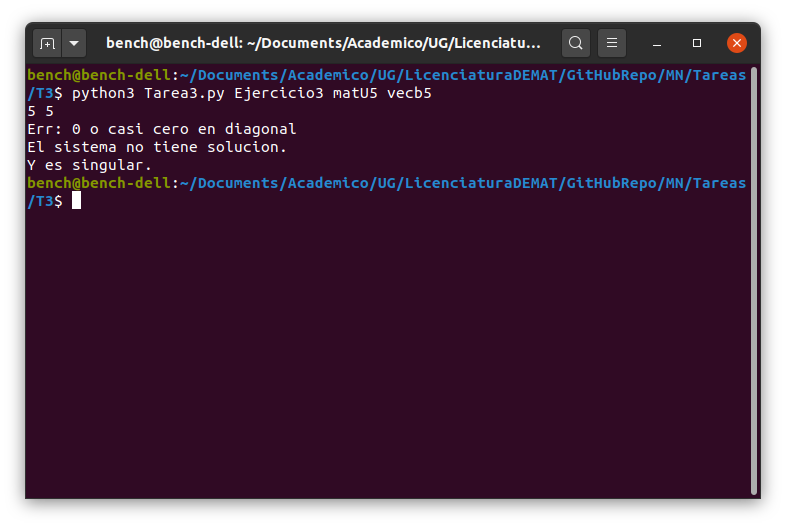
\includegraphics{assets/T3-E3.png}
\caption{Ejemplo ejecucion consola}
\end{figure}


    % Add a bibliography block to the postdoc
    
    
    
\end{document}
